\section{Post synaptic activity due to release of neurotransmitter }

Let it be $p(t)$ the variable of activation of post synaptic currents in a synapse of one synaptic contact which depends on the total of released neurotransmitter. This activation obeys to a lineal dynamic which is given by:

\begin{equation}
\partial_tp = qr\alpha(1-p)-\beta p    
\end{equation}
which can be rewritten as

\begin{equation}
    \partial_tp = \frac{p_{\infty}-p}{\tau_p}
\end{equation}
where 
\begin{equation}
    p_{\infty} = \frac{qr\alpha}{qr\alpha+\beta} 
\end{equation}

and 

\begin{equation}
    \tau_p = \frac{1}{qr\alpha + \beta}
\end{equation}

So the system () is extended to a four dimensional system:

\begin{eqnarray} 
\label{eq : deltap}
\partial_t c &=& \frac{c_{\infty}-c}{\tau_c} + k \sum_{i=1}^n \delta(t-t_i) \\
\partial_t q &=&  \frac{q_{\infty}-q}{\tau_q} - h r q \\
\partial_t r &=& \frac{r_{\infty}(c) - r}{\tau_r}  
\\
\partial_tp &=& \frac{p_{\infty}-p}{\tau_p}
\label{eq : deltapp}
\end{eqnarray}

Using the asymptotic value for $c_n$ (\ref{eq:cAsymptotic}) we can establish a explicit relation between $\tau_c$ and $\tau_r$

\begin{equation}
    \tau_r = \frac{1}{\alpha_r (c_n)^m + \beta_r}
\end{equation} with
\begin{equation}
    c_n = k_c \left(  \frac{1-e^{\frac{-\delta(n+1)}{\tau_c}}}{1-e^{\frac{-\delta}{\tau_c}}}\right)
\end{equation}

So 
\begin{equation}
    \tau_r = \left[ \alpha k_c \left(\frac{1-e^{\frac{-\delta(n+1)}{\tau_c}}}{1-e^{\frac{-\delta}{\tau_c}}}\right)^m - \beta \right]^{-1} 
\end{equation}
So $\tau_r$ depends on $\tau_c$ according to fig().

\begin{figure}
    \centering
    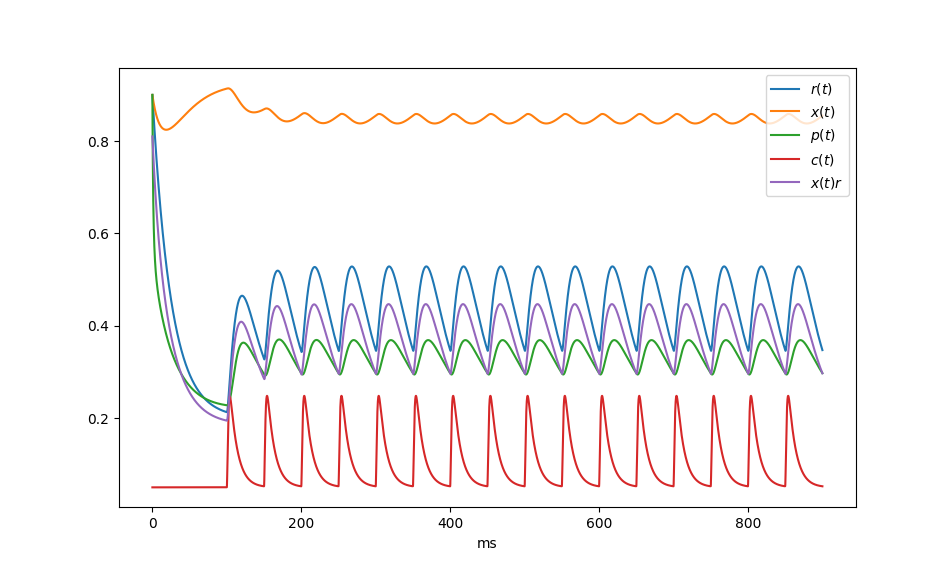
\includegraphics[scale = 0.6]{FacPre_bifPos.png}
    \caption{respuesta bifásica posináptica a pesar de haber facilitación en la liberación de neurotransmisor $xr$}
    \label{fig:my_label}
\end{figure}

\begin{figure}
    \centering
    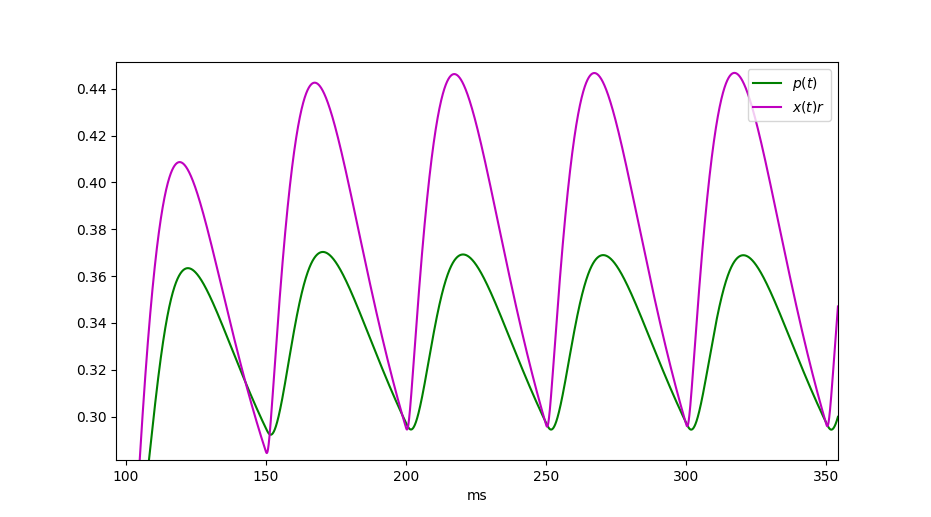
\includegraphics[scale = 0.6]{zoom2.png}
    \caption{zoom de la figura anterior}
    \label{fig:my_label}
\end{figure}

Now, in order to establish a relationship between the rates of recuperation of ready releasable vesicles and the release machinery. We define $L = qr$
Then 
\begin{equation}
    \partial_t L = q \partial_t r + r \partial_t q \\ 
    = q \frac{r_{\infty}(c) - r}{\tau_r} + r \left(\frac{q_{\infty}-q}{\tau_q} - h r q\right)
\end{equation}

The equilibrium state of this variable of release of neurotransmitter give us:  
\begin{equation}
    0 = q \partial_t r + r \partial_t q \\ = q \left(\frac{r_{\infty}(c) - r}{\tau_r}\right) + r \left(\frac{q_{\infty}-q}{\tau_q} - h r q\right)
\end{equation}
which implies that: 
\begin{equation}
     -\frac{r q_{\infty}}{\tau_q}  = q \left(\frac{r_{\infty} - r}{\tau_r} - r( \frac{1}{\tau_q} + h r ) \right)
\end{equation}
So 
\begin{equation}
     q = \frac{-\frac{r q_{\infty}}{\tau_q}}{\left(\frac{r_{\infty} - r}{\tau_r} - r( \frac{1}{\tau_q} + h r ) \right)}  
\end{equation}
